\documentclass[10pt,letterpaper,twocolumn,twoside]{article}
\usepackage[utf8]{inputenc}
\usepackage{amsmath}
\usepackage{amsfonts}
\usepackage{amssymb}
\usepackage{graphicx}
\usepackage[width=0.00cm, height=0.00cm, left=1.00in, right=1.00in, top=1.00in, bottom=1.00in]{geometry}
\author{Phillip Summers, Daniel Chen}
\title{PathLinker 2.0\\Midterm Report}
\begin{document}
	\maketitle
\section{Motivation}

We seek to develop a computational method to automatically construct
signaling pathways using both a background interactome and incomplete
information of the targeted pathway through manual curation.  Ideally
this method should outperform similar techniques which utilize only
the background interactome without the manually curated information.
Performance is measured by the ability to reconstruct a gold standard
signaling pathway while minimizing the number of false positives.

\section{Background}

Signaling pathways are a fundamental aspect of systems biology, they
control how a cell responds to external stimuli and ultimately what
genes are expressed.  Understanding these complex systems guide what
future biological experiments will be most illuminating, while also
suggesting potential pharmaceutical targets.  There exist multiple
databases which store information on cellular interactions, but
curating these interactions into meaningful pathways has traditionally
been a costly manual process.  There exist methods to computationally
predict these pathways, though informative, they are far from perfect.


\subsection{Why are you doing it}

By leveraging computational methods on readily available information
from interaction databases, we are able to reduce the need for
painstaking manual curation.  Computationally constructed signaling
pathways can accelerate the manual curation process, while also
revealing potentially novel connections that human curators may have
overlooked.  These constructed signaling pathways can then guide
experimentalists on what interactions may be most interesting to
study.

%\section{Related previous research}

%Previous methods
%\begin{itemize}
%	\item Pathlinker
%	\item Response Net
%	\item Page Rank
%	\item PCSF
%	\item IPA
%	\item BowTie Builder
%\end{itemize}

\section{What makes your angle different from other approaches}

While predicting pathways, we've previously only considered the
confidence that an interaction takes place through experimental means
(Bayesian approach that computes interaction probabilities based on
sources of evidence).  Edge weights become more informative when we
not only consider the confidence of the interaction, but whether it
has already been curated for our pathway of interest manually.

\section{Approach}

We use a preprocessing step of the interactome originally used in
Pathlinker, altering edge weights based of if that interaction is
passed as known or not.  Edges which are considered known have their
edge weight (probability of interaction) increased, while edges which
are unknown have their edge weight decreased.  As per the original
Pathlinker, these weights are then negative log transformed, then a
k-shortest-paths algorithm is then run on this resulting interactome
utilizing a super-source and super-target.

We intend to use multiple weighting schemes to see which has the best
performance on the wnt pathway.  It should be noted that the precision
recall curve calculation must be altered from the original
Pathlinker's formulation.  Recall of interactions we already passed
the algorithm is not informative, thus we should only use the portion
of the known WNT pathway we withed from Pathlinker 2.0 as the gold
standard.

The planned weighting scheme goes as follows:

\begin{tabular}{cc}
	Not in & In \\ 
	0.1 & 150\% \\ 
	25\% & 200\% \\ 
	50\% & 300\% \\ 
	75\% & 0.9
\end{tabular} 

Where each pairwise set of re-weighting schemes will be calculated

\section{Data}

We are using the NetPath database, and using edge weights as
calculated in the original Pathlinker before our introduced
preprocessing.  In terms of the orignal Pathlinker masterscript, we
used the "--onlynetpathwnt" option.  Precision recall curves
calculated based on a k=10,000 for Pathlinker and Pathlinker2.0,
parameters for other algorithms are left at default values.

\section{Progress}

We have randomly split the edges of the known WNT pathway into two
halves, and stored them as seperate files.  We have developed a
function that takes one of these files, and the interactome, and
outputs a new interactome modified by an edge weight rule.  We have
created 16 such transformed interactomes with which we intend to run
Pathlinker2.0 using each, as a form of parameter scan over our rule
sets.  We have modified the original Pathlinker "masterscript.py" to a
"masterscript2.0.py", and successfully ran the script using one of our
re-weighted interactomes for Pathlinker2.0.  Other algorithms were
passed the orginal interactome without any preprocessing on our part.
From here we printed a precision recall curve comparing Pathlinker2.0
to other algorithms.

The weighting scheme we first ran was the most 'extreme', in that it
weighted a known edge as having a confidence of 0.9 and every other
edge as 0.1.  Other weighting schemes use a multiplier on the original
edge confidence. This retains the Baysian information that is lost in
our initial proof-of-concept strategy (0.9 or 0.1 only).

\vfill
\pagebreak

\section{Preliminary results}

We have run Pathlinker2.0 passing it half of the known WNT pathway,
comparing its precision recall curve to that of: PageRank, Pathlinker,
and BowTieBuilder.  While Pathlinker2.0 outperforms these other
algorithms, however the curve is misleading as this is refering to the
whole wnt pathways as its gold standard.  To account for this
inflation of results, we need to rerun the precesion recall
calculations using only the held out portion of the WNT pathway as the
gold standard.

\vfill
\newpage
\pagebreak
\clearpage

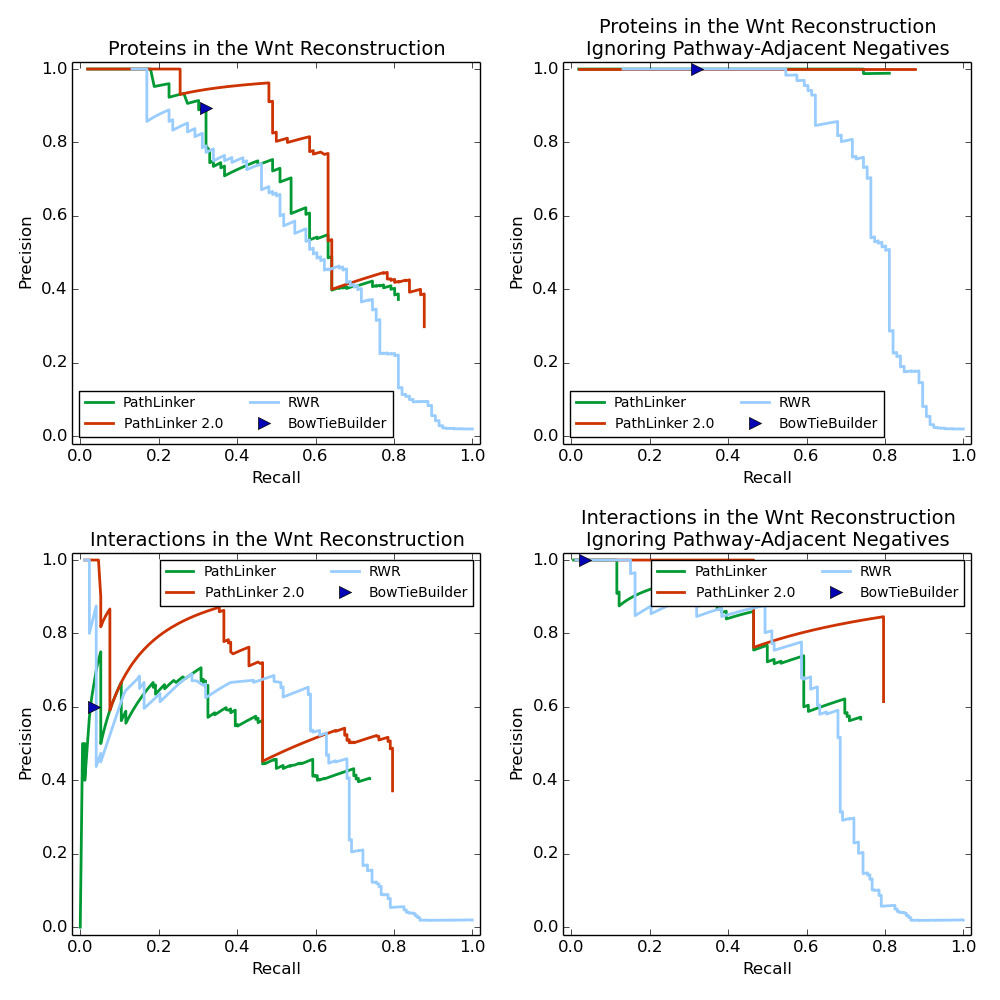
\includegraphics[width=\textwidth]{../midterm_presentation/midterm_results}


\end{document}